\section{1. Linear Equations and Matrices}
% ========================================

\subsection{Solving linear systems}
% ---------------------------------

\subsubsection{Exercises 1.1 2f} 
% ...............................

\begin{equation}\label{eq:ex2f}
    \begin{matrix}
    e x - e y = 2 \\
    e x + e y = 0
    \end{matrix}
\end{equation}

\begin{verbatim}
x, y= symbols('x y', real= true)
eq1= Eq(E*x - E*y, 2)
eq2= Eq(E*x + E*y, 0)
sols= solve([eq1, eq2])
\end{verbatim}

Solved for:

\begin{equation}\label{eq:ex2fsol}
\begin{Bmatrix}x : e^{-1}, & y : - \frac{1}{e}\end{Bmatrix}
\end{equation}

Check solutions by substituting them in the original equations \ref{eq:ex2f}

\begin{verbatim}
eq1.subs(sols)
True
eq2.subs(sols)
True
\end{verbatim}

Solve the system \ref{eq:ex2f} using matrix notation

\begin{verbatim}
coeffs= Matrix([[E, -E], [E, E]])
const= Matrix([2, 0])
[coeffs, const]
\end{verbatim}

\begin{equation}
\begin{bmatrix}\left[\begin{matrix}e & - e\\e & e\end{matrix}\right], & \left[\begin{matrix}2\\0\end{matrix}\right]\end{bmatrix}
\end{equation}

If everything is correct, solutions are consistent with \ref{eq:ex2fsol}:

\begin{verbatim}
coeffs.solve(const)
\end{verbatim}

\begin{equation}
\left[\begin{matrix}e^{-1}\\- \frac{1}{e}\end{matrix}\right]
\end{equation}

\subsubsection{Exercises 1.1 4a}
Plot the graphs of these linear equations
% .....................................................

\begin{equation}
\begin{matrix}2 x + y = 3\\x - y = 7\end{matrix}
\end{equation}

\begin{verbatim}
eq1= Eq(2*x + y, 3)
eq2= Eq(x - y, 7)
\end{verbatim}

Plot

\begin{verbatim}
pp1= plot_implicit(eq1)
pp2= plot_implicit(eq2)
pp1.extend(pp2)
pp1.save('figs/ex4a.pdf')
\end{verbatim}

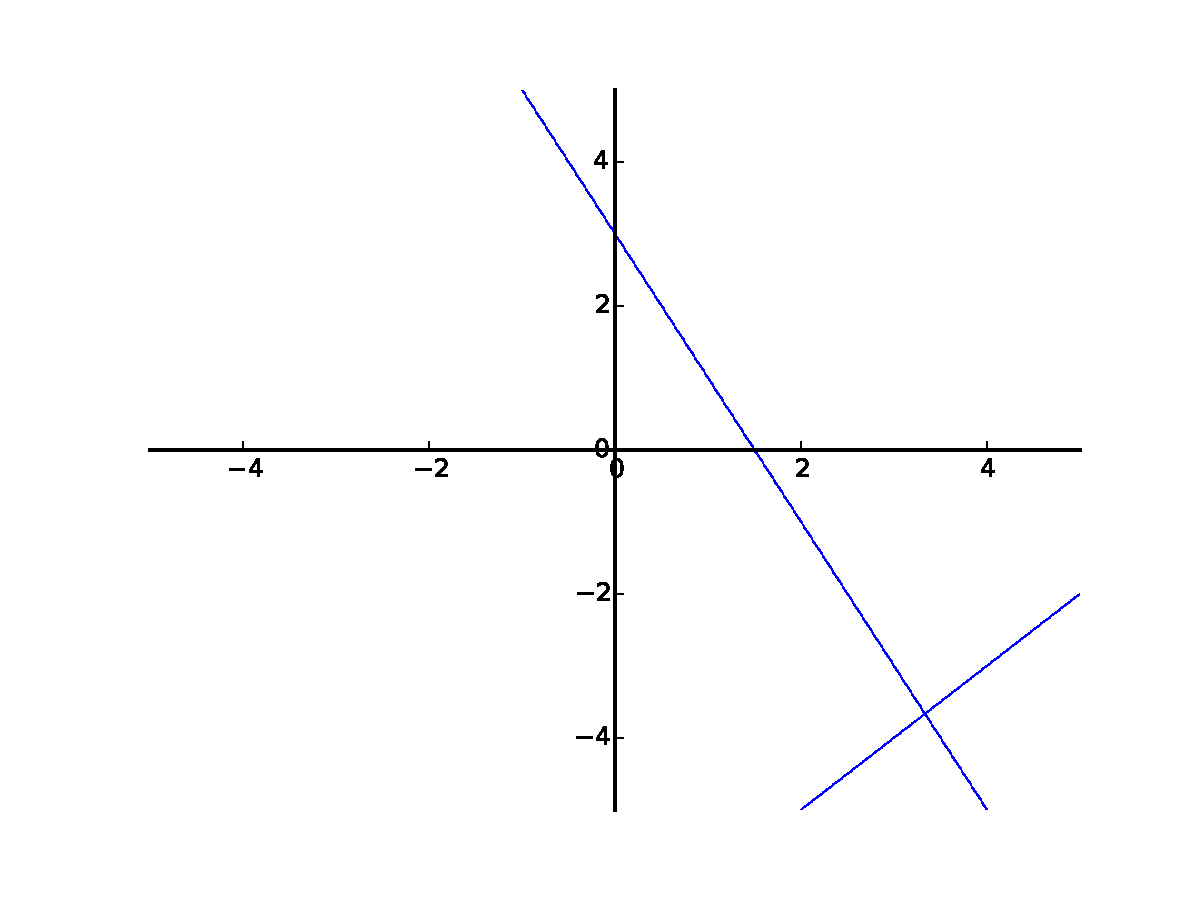
\includegraphics[width=\linewidth]{figs/ex4a.pdf}

\textbf{Exercises 1.1 5b}
% ............

\begin{verbatim}
eq1= Eq(12*x + 4*y, 16)
eq2= Eq(8*x + 4*y, 16)

pp1= plot_implicit(eq1)
pp2= plot_implicit(eq2)
pp1.extend(pp2)
pp1.save('figs/ex5b.pdf')
\end{verbatim}

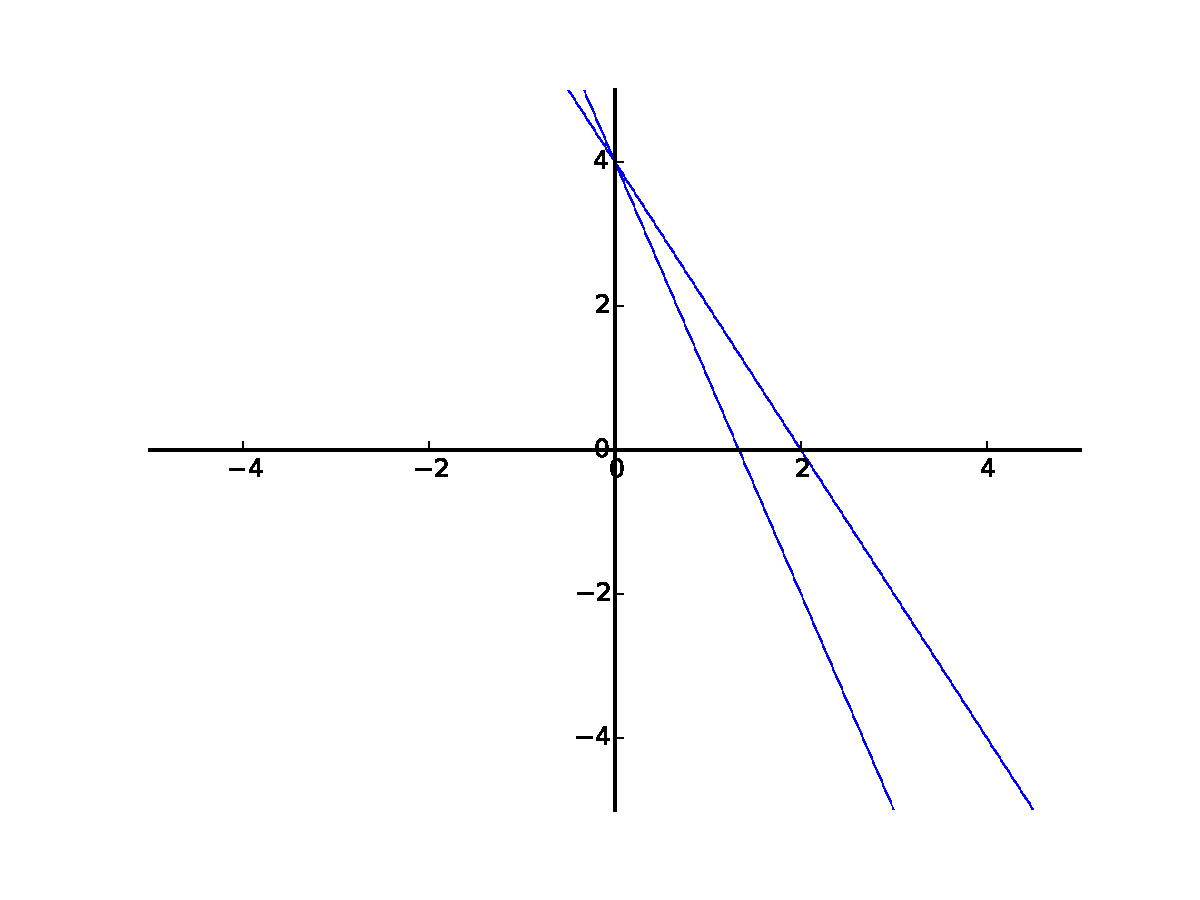
\includegraphics[width=\linewidth]{figs/ex5b.pdf}

\subsection{Solve by row echelon form}
% ------------------------------------

Given a linear system of equations, the solutions can be found by Gaussian
elimination:

\begin{itemize}
\item Extract the coefficients and constants from the equations and put them in
an augmented matrix.
\item Transform the augmented matrix in reduced row echelon form (rref). This is
the result of the Gaussian elimination process.
\item The last columns of the rref matrix lists the solutions of the linear system.
\end{itemize}

Reminder: rref means that every leading coefficient is 1 and is the only nonzero
entry in its column \footnote{http://en.wikipedia.org/wiki/Row\_echelon\_form}. 

\subsubsection{Exercises 1.2 2a}

\begin{equation}
\begin{matrix}x + 2 y + 3 z = 12\\2 x - y + 5 z = 3\\3 x + 3 y + 6 z = 21\end{matrix}
\end{equation}

\begin{verbatim}
eq1= Eq(x + 2*y + 3*z, 12)
eq2= Eq(2*x - y + 5*z, 3)
eq3= Eq(3*x + 3*y + 6*z, 21)
\end{verbatim}

Represent the linear systen as \textit{augmented} matrix, where the last column
holds the constants:

\begin{equation}
M= \left[\begin{matrix}1 & 2 & 3 & \textit{12}\\
                       2 & -1 & 5 & \textit{3}\\
                       3 & 3 & 6 & \textit{21}\end{matrix}\right]
\end{equation}

In \sympy use the \href{http://docs.sympy.org/latest/modules/polys/reference.html#sympy.polys.polytools.Poly}{\texttt{Poly}}
class to conveniently extract the coefficients at the left hand side of
the equations:

\begin{verbatim}
M= Matrix([
    Poly(eq1.lhs).coeffs(),
    Poly(eq2.lhs).coeffs(),
    Poly(eq3.lhs).coeffs()
])
const= Matrix([eq1.rhs, eq2.rhs, eq3.rhs])
M= const.col_insert(0, M)
\end{verbatim}

In reduced row echelon form, with indexes of the pivot variables on the right:

\begin{equation}
RREF= \begin{pmatrix}\left[\begin{matrix}1 & 0 & 0 & 1\\0 & 1 & 0 & 4\\0 & 0 & 1 & 1\end{matrix}\right], & \begin{bmatrix}0, & 1, & 2\end{bmatrix}\end{pmatrix}
\end{equation}

Solutions can be read from last column of the RREF $\left[\begin{matrix}x:1\\y:4\\z:1\end{matrix}\right]$. Verify the solutions solve
the initial system of equations:

\begin{verbatim}
rref= M.rref()
sols= rref[0].col(-1)

eq1.subs({x:sols[0], y:sols[1], z:sols[2]}) # True
eq2.subs({x:sols[0], y:sols[1], z:sols[2]}) # True
eq3.subs({x:sols[0], y:sols[1], z:sols[2]}) # True

# Or the same returning dict {x: 1, y: 4, z: 1}
solve([eq1, eq2, eq3]) 
\end{verbatim}

\subsubsection{Exercises 1.2 3d}
% ..............................

Linear system:

\begin{equation}
\begin{matrix}
    - 2 x + 3 y - 2 z = 8 \\
    - x + 2 y - 10 z = 0 \\
    5 x - 7 y + 4 z = -20
\end{matrix}
\end{equation}

Augmented matrix:

\begin{equation}
\left[\begin{matrix}-2 & 3 & -2 & 8\\-1 & 2 & -10 & 0\\5 & -7 & 4 & -20\end{matrix}\right]
\end{equation}

Reduced row echelon form with solutions in the last column:

\begin{equation}
\begin{pmatrix}\left[\begin{matrix}1 & 0 & 0 & -3 \\
                                   0 & 1 & 0 & 1 \\
                                   0 & 0 & 1 &
\frac{1}{2}\end{matrix}\right], & \begin{bmatrix}0, & 1, & 2\end{bmatrix}\end{pmatrix}
\end{equation}

In \sympy:

\begin{verbatim}
eq1= Eq(-2*x + 3*y -2*z, 8)
eq2= Eq(-x + 2*y - 10*z, 0)
eq3= Eq(5*x - 7*y + 4*z, -20)

M= Matrix([
    Poly(eq1.lhs).coeffs(),
    Poly(eq2.lhs).coeffs(),
    Poly(eq3.lhs).coeffs()
])
const= Matrix([eq1.rhs, eq2.rhs, eq3.rhs])
M= const.col_insert(0, M)
rref= M.rref()
sols= rref[0].col(-1)

# Checked: {x: -3, y: 1, z: 1/2}
solve([eq1, eq2, eq3])
\end{verbatim}

\subsection{Vector arithmetic}
% ----------------------------

\subsubsection{Exercise 1.3.1}

Given two vectors:

\begin{verbatim}
va= Matrix([2, 0])
vb= Matrix([2, 1])
\end{verbatim}

plot the results of the operations 

\subsubsection{(a-e)}

\begin{verbatim}
vA= va + vb          # [4 1]
vB= va - vb          # [0 -1]
vC= 3 * va           # [6 0]
vD= -1/2 * vb        # [-1 -0.5]
vE= 3*va - 1/2 * vb  # [5 -0.5]
\end{verbatim}

And plot vectors

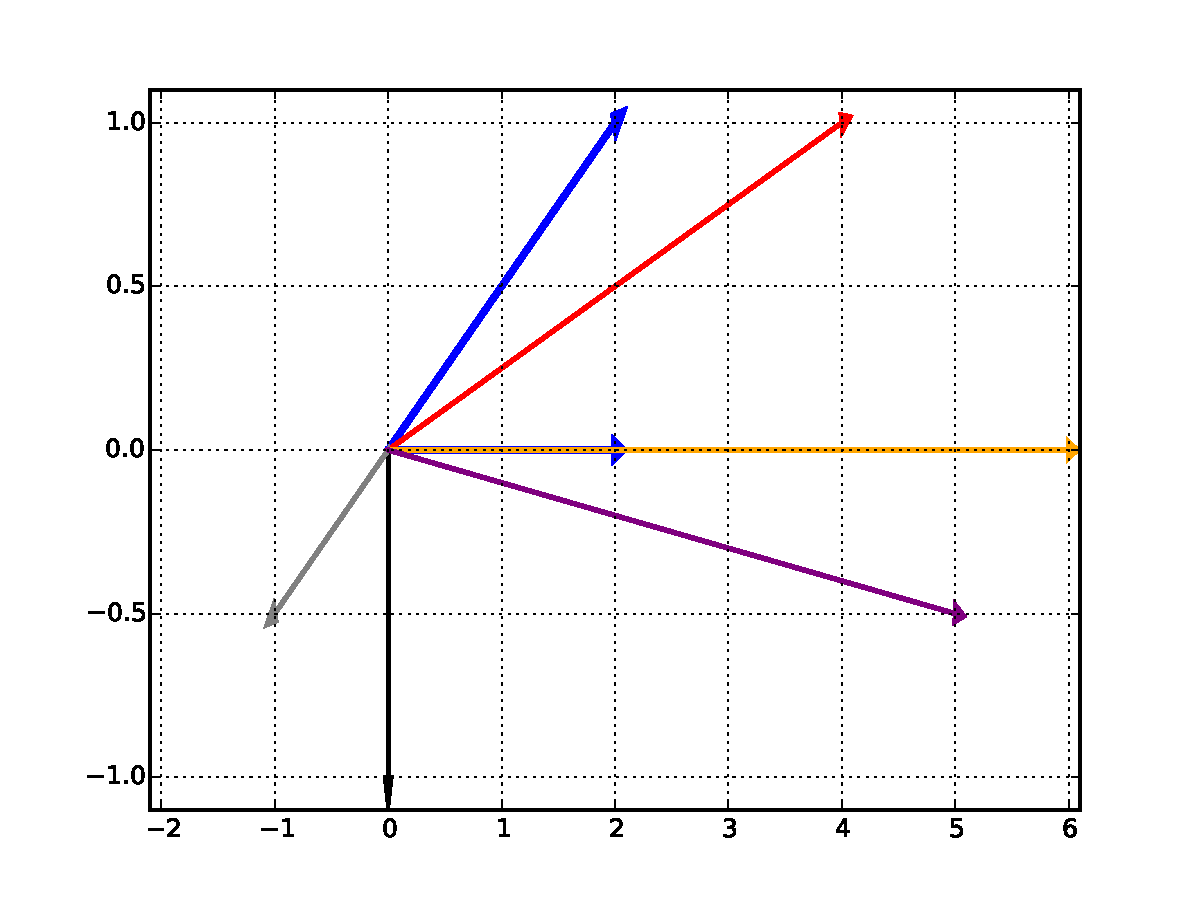
\includegraphics[width=\linewidth]{figs/ex1_3.pdf}

\begin{verbatim}
plt.arrow(0, 0, float(va[0]), float(va[1]), lw= 3, color= 'b', head_width=0.05)
plt.arrow(0, 0, float(vb[0]), float(vb[1]), lw= 3, color= 'b', head_width=0.05)
plt.arrow(0, 0, float(vA[0]), float(vA[1]), lw= 2, color= 'r', head_width=0.05)
plt.arrow(0, 0, float(vB[0]), float(vB[1]), lw= 2, color= 'black', head_width=0.05)
plt.arrow(0, 0, float(vC[0]), float(vC[1]), lw= 2, color= 'orange', head_width=0.05)
plt.arrow(0, 0, float(vD[0]), float(vD[1]), lw= 2, color= 'grey', head_width=0.05)
plt.arrow(0, 0, float(vE[0]), float(vE[1]), lw= 2, color= 'purple', head_width=0.05)
plt.xlim(-2.1, 6.1)
plt.ylim(-1.1, 1.1)
plt.grid()
plt.savefig('figs/ex1_3.pdf')
plt.close()
\end{verbatim}

\subsubsection{Exercise 1.3.8}
% ............................
Show that $x\mathbf{u} + y\mathbf{v} = \mathbf{w}$ where
$\mathbf{u}= (1\ 0)^{T}$, $\mathbf{v}= (0\ 1)^{T}$, and $\mathbf{w}= (x\ y)^{T}$.

This is a consequence of $x(1\ 0) = (x\ 0)$ and $y(0\ 1) = (y\ 0)$. So that
$(x\ 0) + (0\ y) = (x\ y)$

\begin{verbatim}
x, y= symbols('x y')
u= Matrix([1, 0])
v= Matrix([0, 1])
w= Matrix([x, y])
Eq(x*u + y*v, w) # True
\end{verbatim}

\subsubsection{Exercise 1.3.12}
% .............................

Find the real numbers x, y and z, if

\begin{equation}
\left[\begin{matrix}x - 2 z\\2 x + y\\- y + 6 z\end{matrix}\right] = \left[\begin{matrix}5\\3\\17\end{matrix}\right]
\end{equation}

Which is solved for:

\begin{equation}
sols= \begin{bmatrix}\begin{Bmatrix}x : 7, & y : -11, & z : 1\end{Bmatrix}\end{bmatrix}
\end{equation}

\begin{verbatim}
eq1= Eq(x * Matrix([1, 2, 0]) + y * Matrix([0, 1, -1]) + z * Matrix([-2, 0, 6]),
    Matrix([5, 3, 17]))
sols= solve(eq1)
\end{verbatim}

\subsubsection{Exercise 1.3.12}
% .............................

Show that vectors \textbf{u} and \textbf{v} in space $\mathbb{R}^n$ can be
$\mathbf{u} \cdot{} \mathbf{v} = \mathbf{0}$ even if neither \textbf{u} or \textbf{v}
are 0 vectors.

Set:

\begin{verbatim}
u= Matrix([-1, 1])
v= Matrix([1, 1])
u.dot(v) == 0 # True
\end{verbatim}

\subsection{Arithmetic of Matrices}
% ---------------------------------

\subsubsection{Exercise 1.4.1}
% .............................

Given matrix \textbf{B}, note that $3\mathbf{B} = \mathbf{B} + \mathbf{B} + \mathbf{B}$

\begin{equation}
\left[\begin{matrix}6 & -1\\5 & 3\end{matrix}\right]
\end{equation}

\begin{verbatim}
B= Matrix([[6, -1], [5, 3]])
3*B == (B + B + B)
\end{verbatim}

\subsubsection{Exercise 1.4.6}
% .............................

Note how matrx multiplication can result in zero matrix:

\begin{equation}
\left[\begin{matrix}5 & -1 & -2\\10 & -2 & -4\\15 & -3 & -6\end{matrix}\right]
\left[\begin{matrix}1 & 1 & 3\\1 & -1 & -1\\2 & 3 & 8\end{matrix}\right]
= \left[\begin{matrix}0 & 0 & 0\\0 & 0 & 0\\0 & 0 & 0\end{matrix}\right]
\end{equation}

\begin{verbatim}
A= Matrix(3, 3, [5, -1, -2, 10, -2, -4, 15, -3, -6])
B= Matrix(3, 3, [1, 1, 3, 1, -1, -1, 2, 3, 8])
Z= A * B
\end{verbatim}

\subsubsection{Exercise 1.4.8}
% ............................

$\mathbf{x}_n = \mathbf{A}^n\mathbf{x}$ Describes a \textbf{discrete dynamical
system}. Apply this formula to

\begin{equation}\label{eq:ex148}
A = \left[\begin{matrix}0.5 & 0.5\\0.5 & 0.5\end{matrix}\right]
\end{equation}

\begin{verbatim}
A= Matrix(2, 2, [1/2, 1/2, 1/2, 1/2])
\end{verbatim}

For the matrix in \ref{eq:ex148} $A^n = A$:

\begin{verbatim}
A**2 == A # True
A**3 == A # True
A**10 == A # True
\end{verbatim}

matrix in \ref{eq:ex148} is a Markov matrix since the colum sums equal 1.

\subsubsection{Exercise 1.4.10}
% .............................

Determine the image of the matrix \textbf{F} after transformation \textbf{AF}:

\begin{equation}
A = \left[\begin{matrix}1 & 0.2\\0 & 1\end{matrix}\right]
\end{equation}

\begin{equation}
F = \left[\begin{matrix}1 & 1 & 2 & 2 & 1.4 & 1.4 & 2 & 2 & 1.4 & 1.4\\1 & 3 & 3 & 2.6 & 2.6 & 2 & 2 & 1.6 & 1.6 & 1\end{matrix}\right]
\end{equation}

\begin{equation}
AF = \left[\begin{matrix}1.2 & 1.6 & 2.6 & 2.52 & 1.92 & 1.8 & 2.4 & 2.32 & 1.72 & 1.6\\1 & 3 & 3 & 2.6 & 2.6 & 2 & 2 & 1.6 & 1.6 & 1\end{matrix}\right]
\end{equation}

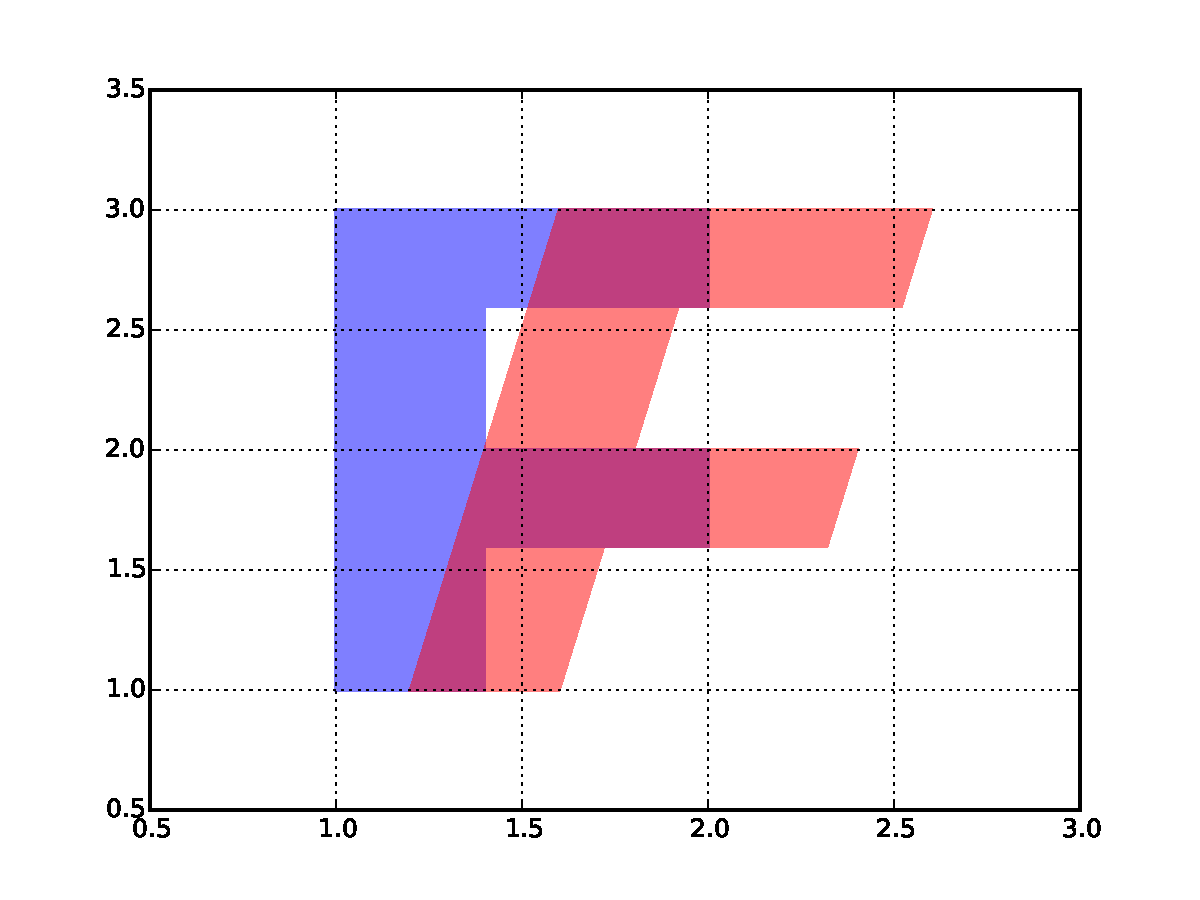
\includegraphics[width=\linewidth]{figs/1_4_10.pdf}

This is showing that the matrix operation $\mathbf{AF} = \mathbf{F_2}$ can be seen as
$\mathbf{f(F)}= \mathbf{F_2}$. That is, the matrix on the left-hand (\textbf{A})
side acts like a function that transforms its argument (\textbf{F}).

\begin{verbatim}
A= Matrix([[1, 0.2], [0, 1]])
F= Matrix([
    [1, 1, 2, 2, 1.4, 1.4, 2, 2, 1.4, 1.4],
    [1, 3, 3, 2.6, 2.6, 2, 2, 1.6, 1.6, 1]])

AF= A*F

verts_F= []
for i in range(F.cols):
    verts_F.append((F[0, i], F[1, i]))
verts_AF= []
for i in range(AF.cols):
    verts_AF.append((AF[0, i], AF[1, i]))

fig = plt.figure()
ax = fig.add_subplot(1, 1, 1)
poly_F = patches.Polygon(verts_F, color= 'b', alpha= 0.5)
poly_AF = patches.Polygon(verts_AF, color= 'r', alpha= 0.5)
ax.set_xlim((0.5, 3))
ax.set_ylim((0.5, 3.5))
ax.add_patch(poly_F)
ax.add_patch(poly_AF)
plt.grid()
plt.savefig('figs/1_4_10.pdf')
\end{verbatim}

\subsubsection{Exercise 1.4.11}
% .............................

\begin{verbatim}
O= Matrix.zeros(2, 1)
X= Matrix([x, y])
\end{verbatim}

\begin{verbatim}
A= Matrix([[1, 2], [3, 5]])
xy= A.solve(O) # x:0, y:0
# Or
xy= A.LUsolve(O) 
# Or
solve(A*X)

A= Matrix([[2, 7], [3, 15]]) # x:0, y:0
xy= A.solve(O)

A= Matrix([[1, 4], [3, 12]]) # Linearly dependent!
xy= A.solve(O)
>>> ValueError: Matrix det == 0; not invertible.
\end{verbatim}

\subsubsection{Exercise 1.4.12}
% .............................

Determine whether vector \textbf{w} is a linear combination of vector \textbf{u}
and \textbf{v}.

Effectively this is asking if the equation $x\mathbf{u} + y\mathbf{v} = \mathbf{w}$
can be resolved.


\begin{itemize}
\item Create an augmented matrix as [u, v, w].
\item Transform the augmented matrix in row echelon form.
\item Get coefficients x and y from last column of RREF. The three vectors are linearly
independent and \textbf{w} $\neq$ \textbf{u} + \textbf{v} (\textbf{w} is not a linear
combination of \textbf{u} and \textbf{v}).

\end{itemize}

\begin{verbatim}
w= Matrix(2, 1, [1, 0])
u= Matrix(2, 1, [5, 8])
v= Matrix(2, 1, [2, 4])
A=  w.col_insert(0, v).col_insert(0, u)
A.rref()
\end{verbatim}

\begin{equation}
REF= \begin{pmatrix}\left[\begin{matrix}1 & 0 & 1\\0 & 1 & -2\end{matrix}\right], & \begin{bmatrix}0, & 1\end{bmatrix}\end{pmatrix}
\end{equation}

\textbf{w} is a linear combination. In fact $1\mathbf{u} -2\mathbf{v}= \mathbf{w}$

\begin{verbatim}
w= Matrix(2, 1, [0, 1])
u= Matrix(2, 1, [5, 8])
v= Matrix(2, 1, [2, 4])
A=  w.col_insert(0, v).col_insert(0, u)
A.rref()
\end{verbatim}

\begin{equation}
\begin{pmatrix}\left[\begin{matrix}1 & 0 & - \frac{1}{2}\\0 & 1 & \frac{5}{4}\end{matrix}\right], & \begin{bmatrix}0, & 1\end{bmatrix}\end{pmatrix}
\end{equation}

\begin{verbatim}
w= Matrix(3, 1, [1, 2, 3])
u= Matrix(3, 1, [1, 0, 0])
v= Matrix(3, 1, [0, 1, 0])
A=  w.col_insert(0, v).col_insert(0, u)
A.rref()
\end{verbatim}

\begin{equation}
REF= \begin{pmatrix}\left[\begin{matrix}1 & 0 & 0\\0 & 1 & 0\\0 & 0 & 1\end{matrix}\right], & \begin{bmatrix}0, & 1, & 2\end{bmatrix}\end{pmatrix}
\end{equation}

\textbf{w} cannot be a linear combination. In fact
$0\mathbf{u} + 0\mathbf{v} \neq [1\ 2\ 3]^T$

\begin{verbatim}
w= Matrix(3, 1, [1, 2, 3])
u= Matrix(3, 1, [4, 8, 0])
v= Matrix(3, 1, [1, 2, -3/7])
A=  w.col_insert(0, v).col_insert(0, u)
A.rref()
\end{verbatim}

\begin{equation}
\begin{pmatrix}\left[\begin{matrix}1 & 0 & 2.0\\0 & 1.0 & -7.0\\0 & 0 & 0\end{matrix}\right], & \begin{bmatrix}0, & 1\end{bmatrix}\end{pmatrix}
\end{equation}

\subsection{Matrix Algebra}
% -------------------------

\subsubsection{Exrcises 1.5.2}
% ............................

Given $A = \left[\begin{matrix}5 & -1 & -2\\1 & -3 & 2\end{matrix}\right]$

A) Find \textbf{B} suc that \textbf{A} + \textbf{B} = \textbf{O} with \textbf{O}
a 2 x 3 matrix.

Requires $\mathbf{A} = \mathbf{B} \Rightarrow \mathbf{B} = -\mathbf{A}$

\begin{verbatim}
A= Matrix([[5, -1, -2], [1, -3, 2]])
O= Matrix.zeros(2, 3)
\end{verbatim}


\subsubsection{Exrcises 1.5.7}
% ----------------------------

Determine the scalar $\lambda$ so that $\mathbf{Ax} = \lambda \mathbf{x}$ with
$\mathbf{A} = \left[\begin{matrix}2 & 1 \\ 1 & 2\end{matrix}\right]$ and $\mathbf{x} = \left[\begin{matrix} 1\\1 \end{matrix}\right]$

$\lambda = 3$ since $\mathbf{Ax} = [3\ 3]^T$.

\begin{verbatim}
A= Matrix([[2, 1], [1, 2]])
x= Matrix(2, 1, [1, 1])
l= symbols('lambda')
solve(Eq(A*x, l*x)) # Lambda= 3
\end{verbatim}

\subsubsection{Exrcises 1.5.10}
% ----------------------------

Given \textbf{T} a transition matrix from a Markov chain and \textbf{p} a
probability vector. Note that the probility vector must sum to 1.

What is the probility that the chain is in a given state after $k$ steps?

The answer is given by $\mathbf{p}_k = \mathbf{T}^k\mathbf{p}$.

For:
\begin{equation}
\left[\begin{matrix}0.6 & 0.7\\0.4 & 0.3\end{matrix}\right]
\end{equation}

\begin{equation}
\left[\begin{matrix}0.5\\0.5\end{matrix}\right]
\end{equation}

Determine $\mathbf{p}_k$ for $k$ in 1, 2, 10, 100, 100000:

$p_{k= 1} = \left[\begin{matrix}0.65\\0.35\end{matrix}\right]$

$p_{k= 2} = \left[\begin{matrix}0.635\\0.365\end{matrix}\right]$

$p_{k= 10} = \left[\begin{matrix}0.63636363635\\0.36363636365\end{matrix}\right]$

$p_{k= 100} = \left[\begin{matrix}0.636363636363634\\0.363636363636362\end{matrix}\right]$

$p_{k= 100000} = \left[\begin{matrix}0.636363636361267\\0.36363636363501\end{matrix}\right]$

Note how the probability vector converges in the long period. The probability vector
at the initial state $k = 0$ might represent the proportion of different species
in the environment. Given the probility of change in \textbf{T}, we can ask the question:
What proportion of species we will see after $k$ iterations (\textit{e.g} generations)?

\begin{verbatim}
T= Matrix(2,2, [0.6, 0.7, 0.4, 0.3])
p= Matrix(2, 1, [0.5, 0.5])
ks= [1, 2, 10, 100, 100000]

for k in ks:
    p_k= T**k * p
    print latex(p_k)
\end{verbatim}


\subsection{Type of solutions}
% ========================================

\subsubsection{Exrcises 1.7.8}
% ----------------------------

\begin{equation}
\textbf{M} = \left[\begin{matrix}1 & 1 & 1 & 0 & 0 & 0 & 6\\0 & 0 & 0 & 1 & 1 & 1 & 15\\1 & 0 & 0 & 1 & 0 & 0 & 5\\0 & 1 & 0 & 0 & 1 & 0 & 7\\0 & 0 & 1 & 0 & 0 & 1 & 9\end{matrix}\right]
\end{equation}

\begin{equation}
\mathbf{M_{rref}}= \begin{pmatrix}\left[\begin{matrix}1 & 0 & 0 & 0 & -1 & -1 & -10\\0 & 1 & 0 & 0 & 1 & 0 & 7\\0 & 0 & 1 & 0 & 0 & 1 & 9\\0 & 0 & 0 & 1 & 1 & 1 & 15\\0 & 0 & 0 & 0 & 0 & 0 & 0\end{matrix}\right], & \begin{bmatrix}0, & 1, & 2, & 3\end{bmatrix}\end{pmatrix}
\end{equation}

There are six variables with coefficents arranged as in matrix $\mathbf{M}$. In
RREF it appears the first four variables, $x_1$ to $x_4$, have 1 as leading
coefficient, as reported by \sympy in the list of pivot variables indexes on the right
(0, 1, 2, 3). Variables $x_5$ and $x_6$ are \textit{free} with coefficients given
in the respective columns. The solutions are therefore:

\begin{equation}
\begin{Bmatrix}x_{1} : x_{5} + x_{6} - 10, & x_{2} : - x_{5} + 7, & x_{3} : - x_{6} + 9, & x_{4} : - x_{5} - x_{6} + 15\end{Bmatrix}
\end{equation}

\begin{verbatim}
M= Matrix([
[1, 1, 1, 0, 0, 0, 6],
[0, 0, 0, 1, 1, 1, 15],
[1, 0, 0, 1, 0, 0, 5],
[0, 1, 0, 0, 1, 0, 7],
[0, 0, 1, 0, 0, 1, 9],
])
M_rref= M.rref()
\end{verbatim}

Solve system of equations:

\begin{verbatim}
x1, x2, x3, x4, x5, x6= symbols('x1:7')
r1= Eq(x1 + x2 + x3, 6)
r2= Eq(x4 + x5 + x6, 15)
r3= Eq(x1 + x4, 5)
c1= Eq(x2 + x5, 7)
c2= Eq(x3 + x6, 9)
sols= solve([r1, r2, r3, c1, c2])
\end{verbatim}

\subsubsection{Exrcises 1.7.11}
% ----------------------------

\begin{verbatim}
x, y, z, t= symbols('x y z t', real= True)

eq1= Eq(2*x - 4*y + 4*z + 0.077*t, 3.86)
eq2= Eq(     -2*y + 2*z - 0.056*t, -3.47)
eq3= Eq(2*x - 2*y,                 0)
sols= solve([eq1, eq2, eq3], [x, y, z])
\end{verbatim}

The solutions \texttt{sols}  are in \ref{eq:ex1_7_11}.

Solving via augmented matrix in reduced row echelon form:

\begin{verbatim}
M= Matrix([
    [2, -4, 4, 0.077, 3.86],
    [0, -2, 2, -0.056, -3.47],
    [2, -2, 0, 0, 0]
])
M_rref= M.rref()
\end{verbatim}

\begin{equation}
\begin{matrix}
2 x - 4 y + 4 z + 0.077 t= 3.86, & \\
- 2 y + 2 z - 0.056 t = -3.47, & \\
2 x - 2 y = 0\end{matrix}
\end{equation}

\begin{equation}
M= \left[\begin{matrix}2 & -4 & 4 & 0.077 & 3.86\\0 & -2 & 2 & -0.056 & -3.47\\2 & -2 & 0 & 0 & 0\end{matrix}\right]
\end{equation}

\begin{equation}
M_{rref} = \begin{pmatrix}\left[\begin{matrix}1 & 0 & 0 & 0.0945 & 5.4\\0 & 1 & 0 & 0.0945 & 5.4\\0 & 0 & 1 & 0.0665 & 3.665\end{matrix}\right], & \begin{bmatrix}0, & 1, & 2\end{bmatrix}\end{pmatrix}
\end{equation}

Note that the 4th column holds the coefficients for the free variable $t$ while the
last column has the values for $x, y, z$. Compare to the solutions
from \sympy \texttt{solve}:

\begin{equation}\label{eq:ex1_7_11}
\begin{Bmatrix}x : - 0.0945 t + 5.4, & y : - 0.0945 t + 5.4, & z : - 0.0665 t + 3.665\end{Bmatrix}
\end{equation}

\subsection{The inverse matrix method}
% ====================================

\subsubsection{Exrcises 1.8.3}
% ----------------------------

What effect has the matrix \textbf{E} on the matrix \textbf{A}. With \textbf{A}
a generic 3x3 matrix:

\begin{verbatim}
x1, x2, x3, x4, x5, x6, x7, x8, x9= symbols('x1:10')
k= symbols('k', zero= False)
A= Matrix(3,3, [x1, x2, x3, x4, x5, x6, x7, x8, x9])
\end{verbatim}

\begin{equation}\label{eq:1_8_3A}
\mathbf{A} = \left[\begin{matrix}x_{1} & x_{2} & x_{3}\\x_{4} & x_{5} & x_{6}\\x_{7} & x_{8} & x_{9}\end{matrix}\right]
\end{equation}

\begin{equation}
\mathbf{E} = \left[\begin{matrix}1 & 0 & 0\\0 & -1 & 0\\0 & 0 & 1\end{matrix}\right]
\end{equation}

\begin{verbatim}
E_a= Matrix([
    [1, 0, 0],
    [0, -1, 0],
    [0, 0, 1]
])
print latex(E_a * A)
\end{verbatim}

\begin{equation}
\mathbf{E_aA} = \left[\begin{matrix}x_{1} & x_{2} & x_{3}\\- x_{4} & - x_{5} & - x_{6}\\x_{7} & x_{8} & x_{9}\end{matrix}\right]
\end{equation}

\begin{verbatim}
E_b= Matrix([
    [0, 0, 1],
    [0, 1, 0],
    [1, 0, 0]
])
print latex(E_b * A)
\end{verbatim}

\begin{equation}
\mathbf{E_bA} = \left[\begin{matrix}x_{7} & x_{8} & x_{9}\\x_{4} & x_{5} & x_{6}\\x_{1} & x_{2} & x_{3}\end{matrix}\right]
\end{equation}

\begin{verbatim}
E_c= Matrix([
    [k, 0, 0],
    [0, 1, 0],
    [0, 0, 1]
])
print latex(E_c * A)
\end{verbatim}

\begin{equation}
\mathbf{E_cA} = \left[\begin{matrix}k x_{1} & k x_{2} & k x_{3}\\x_{4} & x_{5} & x_{6}\\x_{7} & x_{8} & x_{9}\end{matrix}\right]
\end{equation}


\begin{verbatim}
E_d= Matrix([
    [1, 0, 0],
    [0, 1, 0],
    [0, 0, -1/k]
])
print latex(E_d * A)
\end{verbatim}

\begin{equation}
\mathbf{E_dA} = \left[\begin{matrix}x_{1} & x_{2} & x_{3}\\x_{4} & x_{5} & x_{6}\\- \frac{x_{7}}{k} & - \frac{x_{8}}{k} & - \frac{x_{9}}{k}\end{matrix}\right]
\end{equation}

\subsubsection{Exrcises 1.8.5}
% ----------------------------

Solve the linear systems using inverse matrix method.

\begin{equation}\label{eq:eqs_1_8_5}
\begin{matrix}x + 2 y = 3, & \\ - x + 4 y = 5\end{matrix}
\end{equation}

The coefficients on the LHS of the equations can be thought as a matrix
\textbf{A}. \textbf{A} transforms the vector of unknown coefficients \textbf{x}
to produce the vector of constants \textbf{b} on the RHS:

\begin{equation}\label{eq:1_8_5}
\mathbf{A}\mathbf{x} = \mathbf{b}
\end{equation}

To find the vector \textbf{x} we can rearrange \ref{eq:eqs_1_8_5} as:

\begin{equation}
\mathbf{x} = \mathbf{A}^{-1}\mathbf{b}
\end{equation}

In case of \ref{eq:eqs_1_8_5} we have $\mathbf{A} = \left[\begin{matrix}1 & 2\\-1 & 4\end{matrix}\right]$,
$\mathbf{b} = \left[\begin{matrix}3\\5\end{matrix}\right]$. So
$\mathbf{A^{-1}} = \left[\begin{matrix}\frac{2}{3} & - \frac{1}{3}\\\frac{1}{6} & \frac{1}{6}\end{matrix}\right]$
and $\mathbf{x} = \mathbf{A^{-1}b} = \left[\begin{matrix}\frac{1}{3}\\\frac{4}{3}\end{matrix}\right]$

\begin{verbatim}
x, y= symbols('x y')
eq1= Eq(x + 2*y, 3)
eq2= Eq(-x + 4*y, 5)

A = Matrix(2, 2, [1, 2, -1, 4])
b = Matrix(2, 1, [3, 5])
Ai= A.inv()
x= Ai * b
\end{verbatim}

In case of $\mathbf{Ax = b}$ as:

\begin{equation}
\left[\begin{matrix}1 & 0 & 2\\2 & 3 & 1\\3 & 6 & 0\end{matrix}\right]
\mathbf{x} = 
\left[\begin{matrix}-1\\1\\9\end{matrix}\right]
\end{equation}

Matrix \textbf{A} is not invertible and the system has no solutions.

\begin{verbatim}
A = Matrix([
[1, 0, 2],
[2, 3, 1],
[3, 6, 0]
])
b= Matrix(3, 1,  [-1 , 1, 9])

Ai= A.inv()
# ValueError: Matrix det == 0; not invertible.
\end{verbatim}

\subsubsection{Exrcises 1.8.7}
% ----------------------------

\textbf{Leontief input-output model}. Represents the production \textbf{p} and
demand \textbf{d} as a matrix. \textbf{p} and \textbf{d} are vectors where each entry
represents a good. The production of goods is represented as a matrix where each row
states how much units of the other goods (input) is required to produce one unit
of that good (output). With this model we can ask how much input is needed to produce
a given amount of output.

$$
\bordermatrix{\text{}& O & E & S \cr
                 O & 0.25 &  0.15  & 0.1 \cr
                 E & 0.4  &  0.15  & 0.2 \cr
                 S & 0.15 &  0.2   & 0.2} = \mathbf{A}
$$

Reading this matrix row by row, it tells how much Oil, Energy and Services it is
needed to produce one unit of O, E, or S. For example 1 unit of O requires 0.25 units
of O, 0.15 of E and 0.1 units of S.

From this matrix we can relate the production vector \textbf{p} to the demand
vector \textbf{d} as:

\begin{equation}\label{eq:1_8_7io}
\mathbf{p} = \mathbf{Ap} + \mathbf{d}
\end{equation}


We want to know \textbf{p} given \textbf{A} and the demand vector \textbf{d}.
\emph{I.e.} we want to solve \ref{eq:1_8_7io} \emph{w.r.t.} \textbf{p} by re-arranging
to the form \textbf{Ax = b}.

$$\mathbf{
p - Ap = d
}$$

then use the identity matrix to obtain the solvable form \textbf{Ax = b}:

$$\mathbf{
p(I - A) = d
}$$

Now solve by inverting \textbf{(I - A)}:

$$\mathbf{
p = (I - A)^{-1} d
}$$

If the demand for O, E, and S is $\mathbf{d} = [100, 100, 100]^T$ we need to
produce
$\left[\begin{matrix}O \\ E \\ S \end{matrix}\right] = \left[\begin{matrix}220 \\ 276 \\ 235 \end{matrix}\right]$

\begin{verbatim}
A = Matrix([
[0.25, 0.15, 0.1],
[0.4, 0.15, 0.2],
[0.15, 0.2, 0.2]
])

d= Matrix(3, 1, [100, 100, 100])
ii= eye(A.rows)
p= (ii - A).inv() * d
\end{verbatim}



\subsubsection{Exrcises 1.8.8}
% ----------------------------

Show that if \textbf{A} is invertible then $A^Tx=b$ has a unique solution.

\begin{verbatim}
x1, x2, x3, x4, x5, x6, x7, x8, x9= symbols('x1:10')
A= Matrix(3,3, [x1, x2, x3, x4, x5, x6, x7, x8, x9])

k1, k2, k3= symbols('k1:4')
b= Matrix(3, 1, [k1, k2, k3])

A_rref= A.transpose().solve(b).rref()
\end{verbatim}

\begin{equation}
\mathbf{A_{rref}} = \begin{pmatrix}\left[\begin{matrix}1\\0\\0\end{matrix}\right], & \begin{bmatrix}0\end{bmatrix}\end{pmatrix}
\end{equation}

\textit{Does it mean there is a unique solution?}